\subsubsection{Herausforderungen bei der Übernahme und Anpassung}
\label{chap:Herausforderungen bei der Übernahme und Anpassung}

Eine Herausforderung bei der Umsetzung des \ac{c-ep} ist das Finden einer passenden Aktivierungsfunktion für die Zusammenarbeit mit der Lernregel \(\frac{dW_{ij}}{dt}\) und einer passenden Lernrate \(\eta\), welche eine effiziente Konvergenz der Gewichte gewährleistet. Für die bisher gewählte Aktivierungsfunktion, die logistische Funktion wie dargestellt in Abbildung \ref{fig:Graph der Aktivierungsfunktion}, gilt \(\rho(x) > 0\), weshalb auch die Lernregel immer positiv ist. Die Auswirkungen dessen sind in Abbildung \ref{fig:C-EP Non-Negative Aktivierungsfunktion} dargestellt, wobei als Zielwert für das Netzwerk \(\vec{d}=(0,0,0)\) gewählt wurde. Die Ausgabe des Netzwerks richtet sich zu Beginn der zweiten Phase offensichtlich in Richtung der Zielwerte, steigt aber nach einer kurzen Zeit stetig an, da der positive Einfluss der Gewichte den negativen der Kostenfunktion übersteigt.

\begin{figure}[h]
  \label{fig:Graph der Aktivierungsfunktion}
  \caption{Graph der Aktivierungsfunktion \(\rho(x)=\frac{1}{1+e^{-x}}\) (rot) und ihrer Ableitung (grün)}
  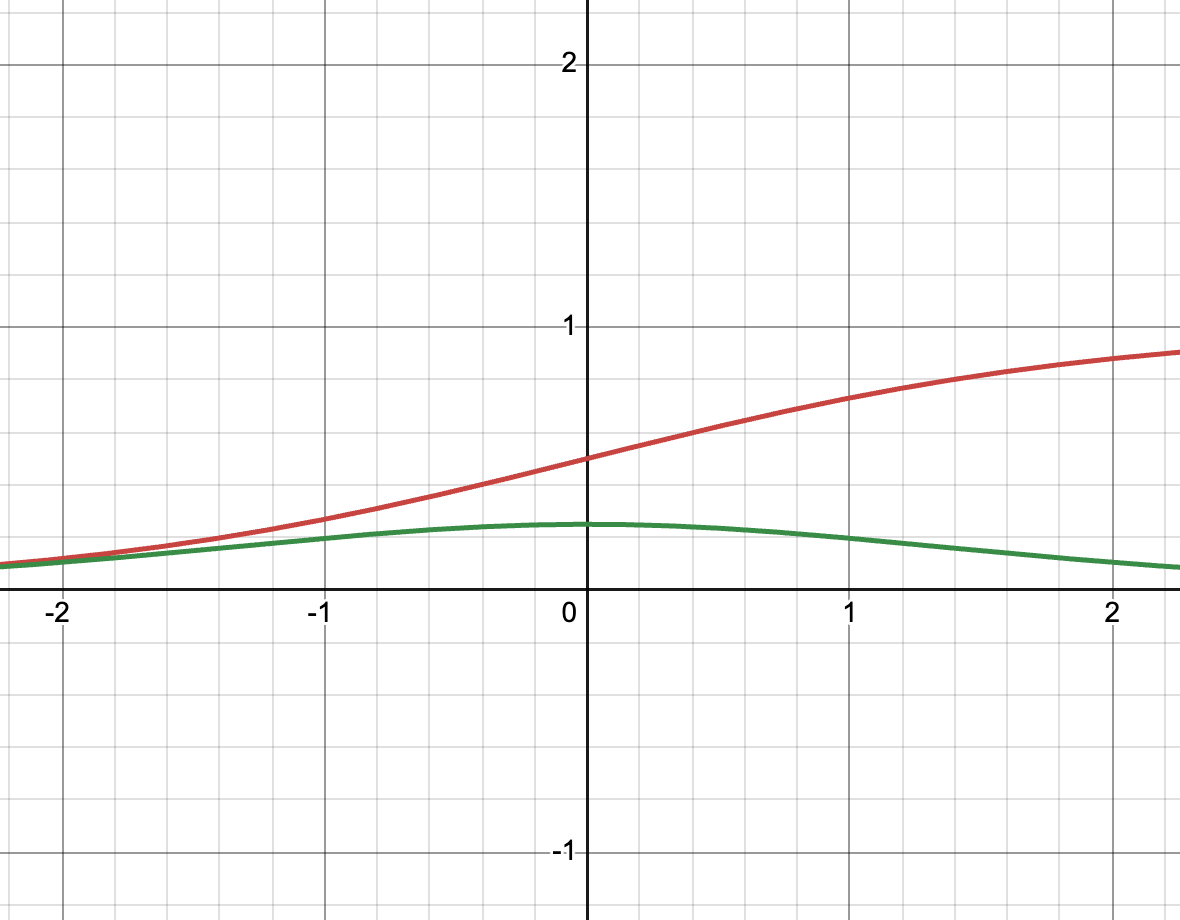
\includegraphics[width=0.5\textwidth]{abbildungen/sigmoid_funktion.png}
  \\
  Quelle: Eigene Darstellung
\end{figure}

\begin{figure}[h]
  \caption{Auswirkungen einer nicht-negativen Aktivierungsfunktion auf das \ac{c-ep}}
  \label{fig:C-EP Non-Negative Aktivierungsfunktion}
  \centering
  \begin{subfigure}[b]{0.5\textwidth}
    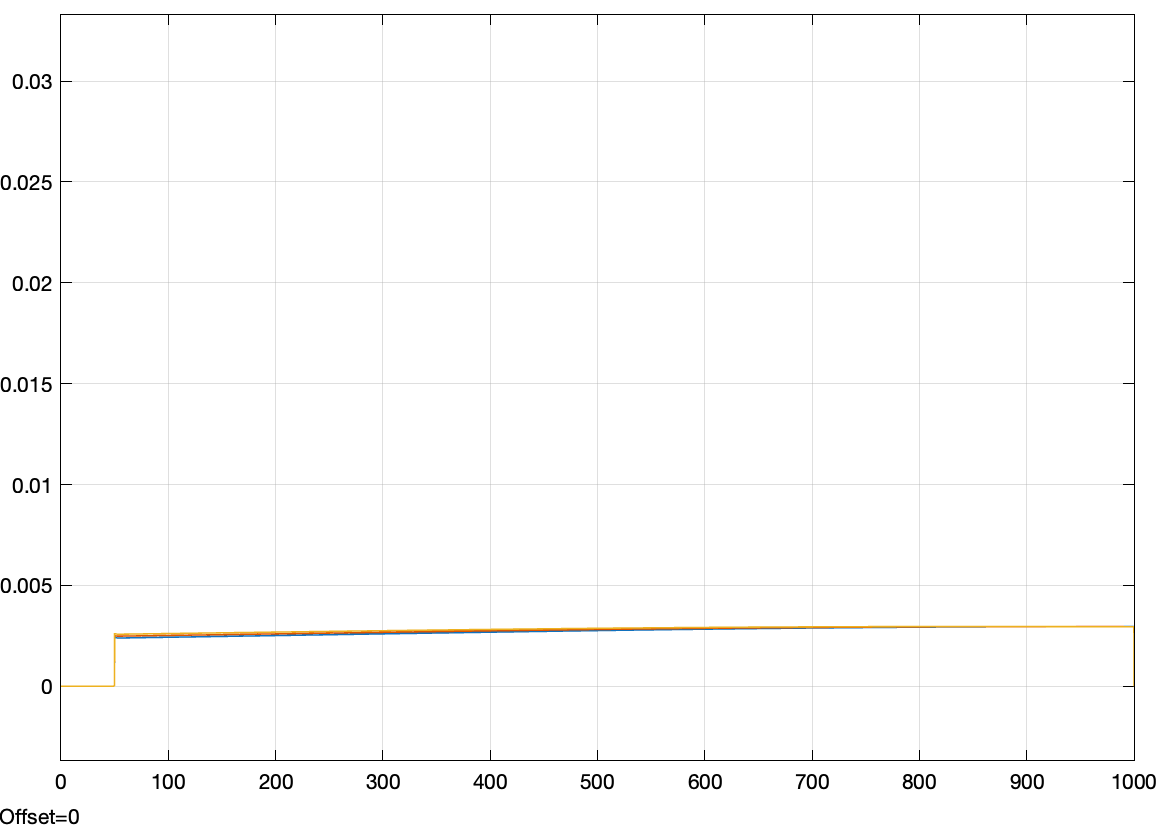
\includegraphics[width=\textwidth]{abbildungen/c_ep_non_negative_activation_weight_update.png}
    \caption{Änderungsrate der Gewichte}
  \end{subfigure}%
  \hfill
  \begin{subfigure}[b]{0.5\textwidth}
    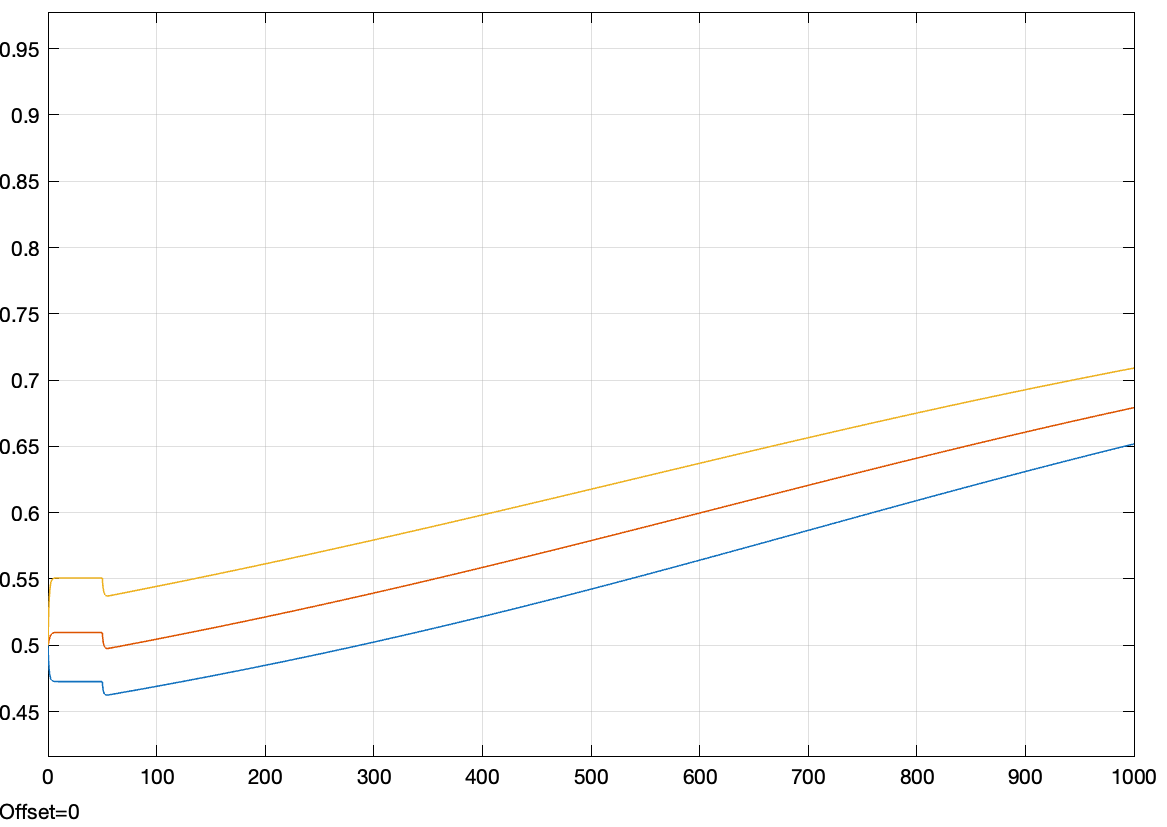
\includegraphics[width=\textwidth]{abbildungen/c_ep_non_negative_activation_ausgabe.png}
    \caption{Ausgabe des Modells}
  \end{subfigure}
  \\
  Quelle: Eigene Darstellung
\end{figure}

Die Dauer der beiden Phasen des \ac{c-ep} wurde durch die Konvergenz dieser definiert. So soll die erste Phase durchgeführt werden bis das Netzwerk einen Fixpunkt findet, für die zweite Phase müssen Fixpunkte des Netzwerkes und der Parameter gefunden werden (\cite[vgl. S. 3]{Ernoult2020}). Die Bestimmung sinnvoller Werte für die Dauer dieser Phasen stellt die Umsetzung des Lernprozesses vor eine weitere Herausforderung. Wie bereits in \ref{chap:Simulation des angepassten Netzwerks} gezeigt, propagiert das implementierte \ac{hnn} mit beliebigem \(\beta\) zuverlässig innerhalb von weniger als zehn Zeiteinheiten zu einem Fixpunkt. Gleiches sollte auf die feste Phase zutreffen, dies ist aber, wie in Abbildung \ref{fig:C-EP Konvergenz Problem} gezeigt, nicht der Fall. Eine mögliche Ursache hierfür stellt erneut die Auswahl der Aktivierungsfunktion dar, da, wie aus Abbildung \ref{fig:Graph der Aktivierungsfunktion} abzulesen, \(\rho(x) > 0\) bzw. \(\dot{\rho}(x) > 0\) und somit \(\frac{dW_{ij}}{dt} > 0\) gilt. Eine Simulation mit \(\vec{d}=(0.8,0.8,0.8)\) und \(\eta=0.1\) zeigt die valide Anpassung der Gewichte bis zu einem Zeitpunkt \(t\approx250\) aber die anschließende fehlende Konvergenz der Parameter.

\begin{figure}[h]
  \label{fig:C-EP Konvergenz Problem}
  \caption{Die Parameter des Modells gelangen zu keinem Fixpunkt und verfehlen damit das Minimum der Kostenfunktion}
  \centering
  \begin{subfigure}[b]{0.3\textwidth}
    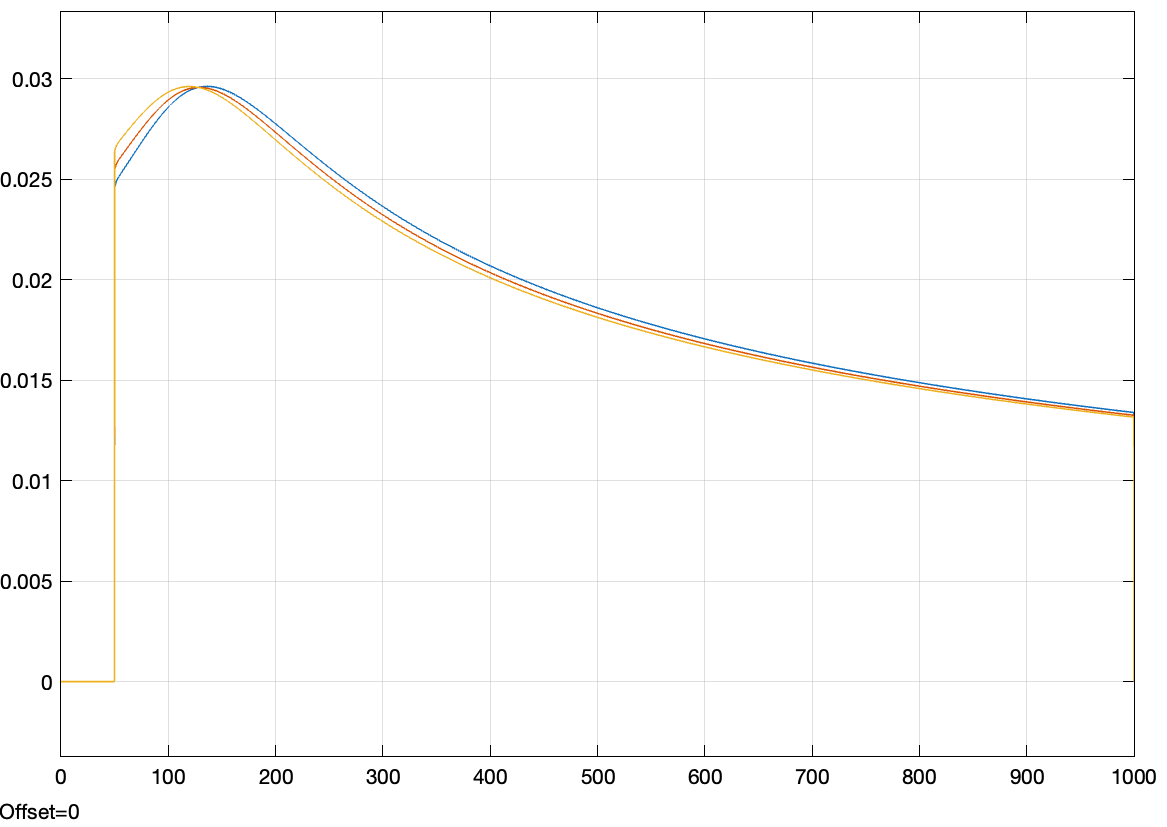
\includegraphics[width=\textwidth]{abbildungen/c_ep_convergence_weight_update.png}
    \caption{Änderungsrate der Gewichte}
  \end{subfigure}%
  \hfill
  \begin{subfigure}[b]{0.3\textwidth}
    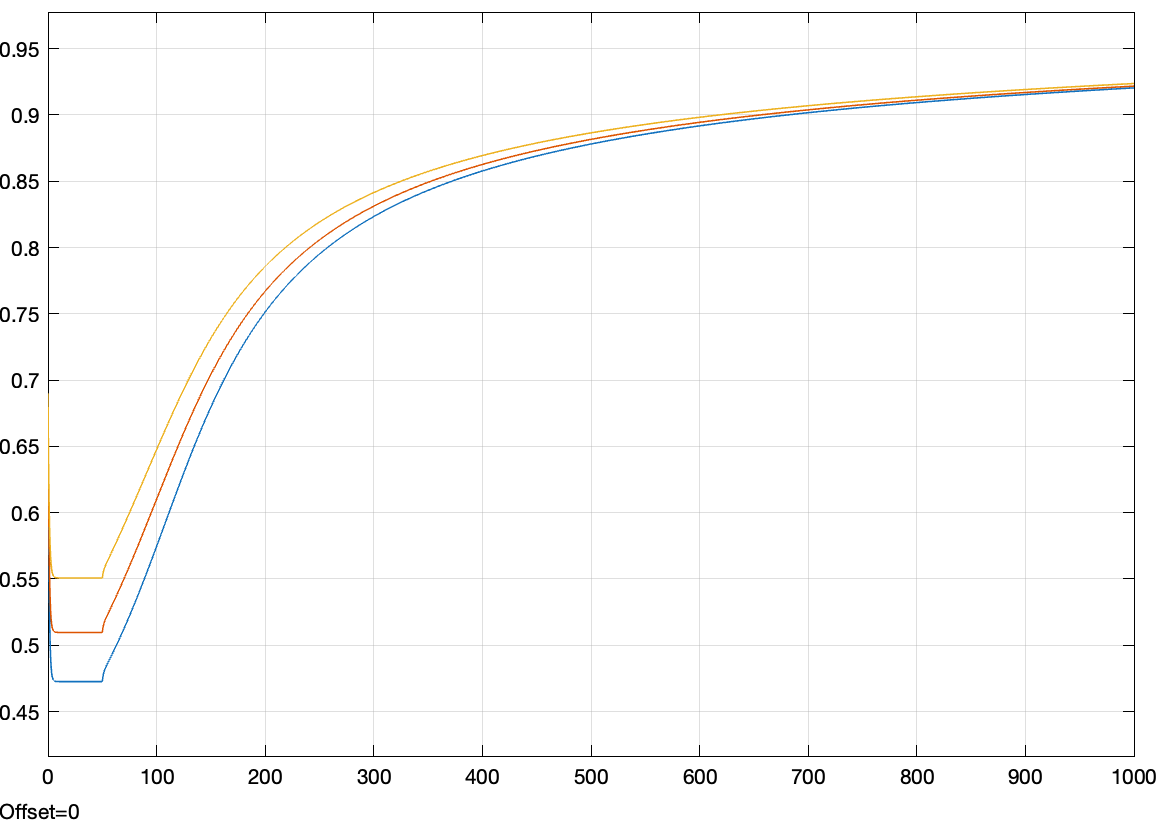
\includegraphics[width=\textwidth]{abbildungen/c_ep_convergence_ausgabe.png}
    \caption{Ausgabe des Modells}
  \end{subfigure}%
  \hfill
  \begin{subfigure}[b]{0.3\textwidth}
    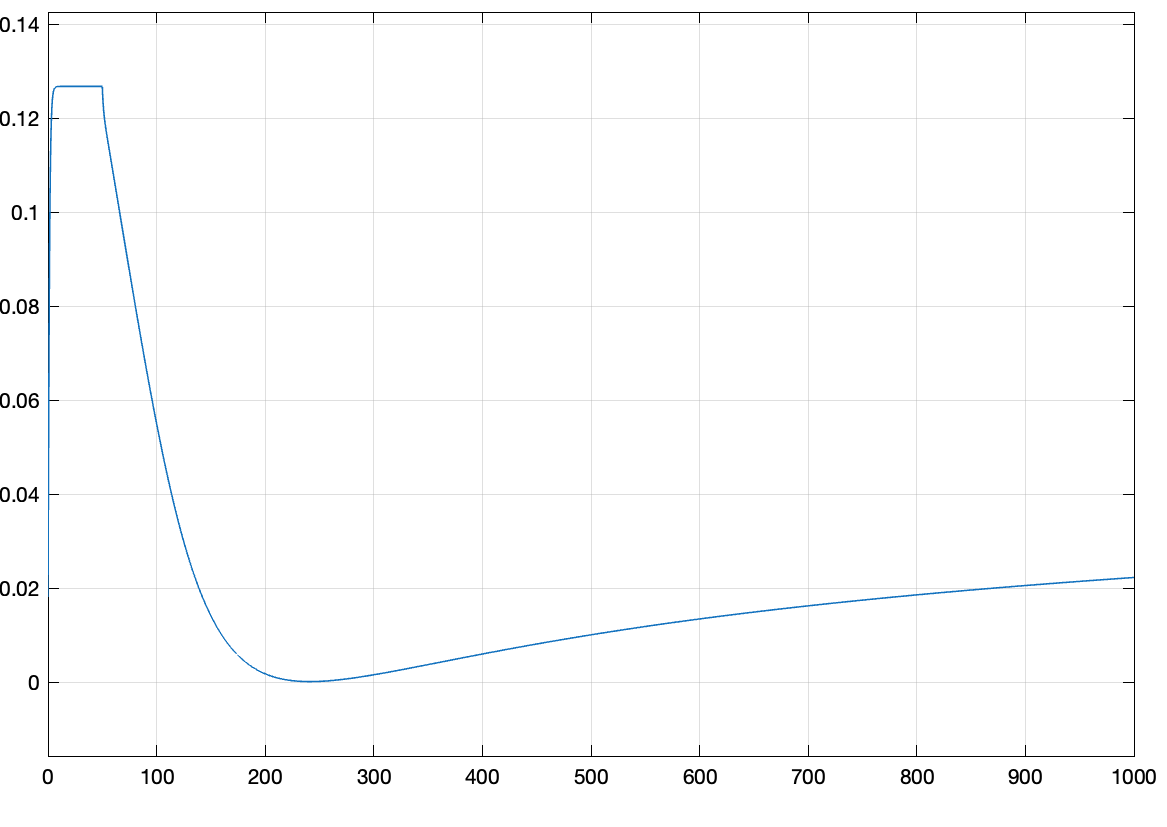
\includegraphics[width=\textwidth]{abbildungen/c_ep_convergence_kosten.png}
    \caption{Kosten des Modells}
  \end{subfigure}
  \\
  Quelle: Eigene Darstellung
\end{figure}

Um Fehler bei der Auswahl der Aktivierungsfunktion oder der Übernahme der Lernregel auszuschließen, wird im Folgenden die von \citeauthor{Ernoult2020} ursprünglich für \ac{c-ep} vorgestellte Lernregel verwendet:

\[\Delta^{C-EP}_{Wnn+1}(\beta,\eta,t)=\frac{1}{\beta}\left(\sigma\left(s^{n,\beta,\eta}_{t+1}\right)\sigma\left(s^{n+1,\beta,\eta}_{t+1}\right)^\intercal-\sigma\left(s^{n,\beta,\eta}_{t}\right)\sigma\left(s^{n+1,\beta,\eta}_{t}\right)^\intercal\right)\]

Angewandt auf das hier genutzte \ac{hnn} und unter Beachtung der Lernrate \(\eta\) ergibt sich:

\[\Delta^{C-EP}_{W_{ij}}(\eta,t)\propto\eta\left(\rho(u^{\beta}_{t+1,i})\rho(u^{\beta}_{t+1,j})-\rho(u^{\beta}_{t,i})\rho(u^{\beta}_{t,j})\right)\]

\[\Delta^{C-EP}_{b_{i}}(\eta,t)\propto\eta\left(\rho(u^{\beta}_{t+1,i})-\rho(u^{\beta}_{t,i})\right)\]

Anhand dieser Lernregel kann die Dynamik \(\frac{dW_{ij}}{dt}\) approximiert werden, indem praktisch mit einer Zeitverschiebung gearbeitet wird. Simulink bietet hierfür den Block "`Transport Delay"', welcher ein kontinuierliches Eingangssignal um einen beliebigen Zeitraum verschiebt. Die Zeitverschiebung ist kein grundlegender Bestandteil herkömmlicher analoger Computer (siehe Kapitel \ref{chap:Typische Komponenten und Bauweisen analoger Computer}) und für diese Aufgabe eignet sich auch wieder ein hybrider Ansatz, da Informationen (auch wenn nur über einen sehr kurzen Zeitraum) gespeichert werden müssen. Es existieren aber auch Ansätze zur Annäherung einer Zeitverschiebung auf analoger Hardware (\cite[vgl. S. 117 ff.]{Ulmann2022}). Negative Gewichtsanpassungen sind mit diesem Ansatz ohne weiteres möglich und der beispielhafte Durchlauf des Netzwerks mit \(\vec{d}=(0.8,0.8,0.8)\) (jetzt mit \(\eta=10\)) konvergiert mit diesem Ansatz zu sinnvollen Gewichten (siehe Abbildung \ref{fig:C-EP Annäherung Konvergenz}). Im Anhang \ref{app:Umsetzung des Equilibrium-Propagation in Simulink} wird das Simulink-Modell zu diesem Ansatz gezeigt.

\begin{figure}[h]
  \label{fig:C-EP Annäherung Konvergenz}
  \caption{Eine Annäherung an C-EP findet passende Parameter für das Netzwerk}
  \centering
  \begin{subfigure}[b]{0.3\textwidth}
    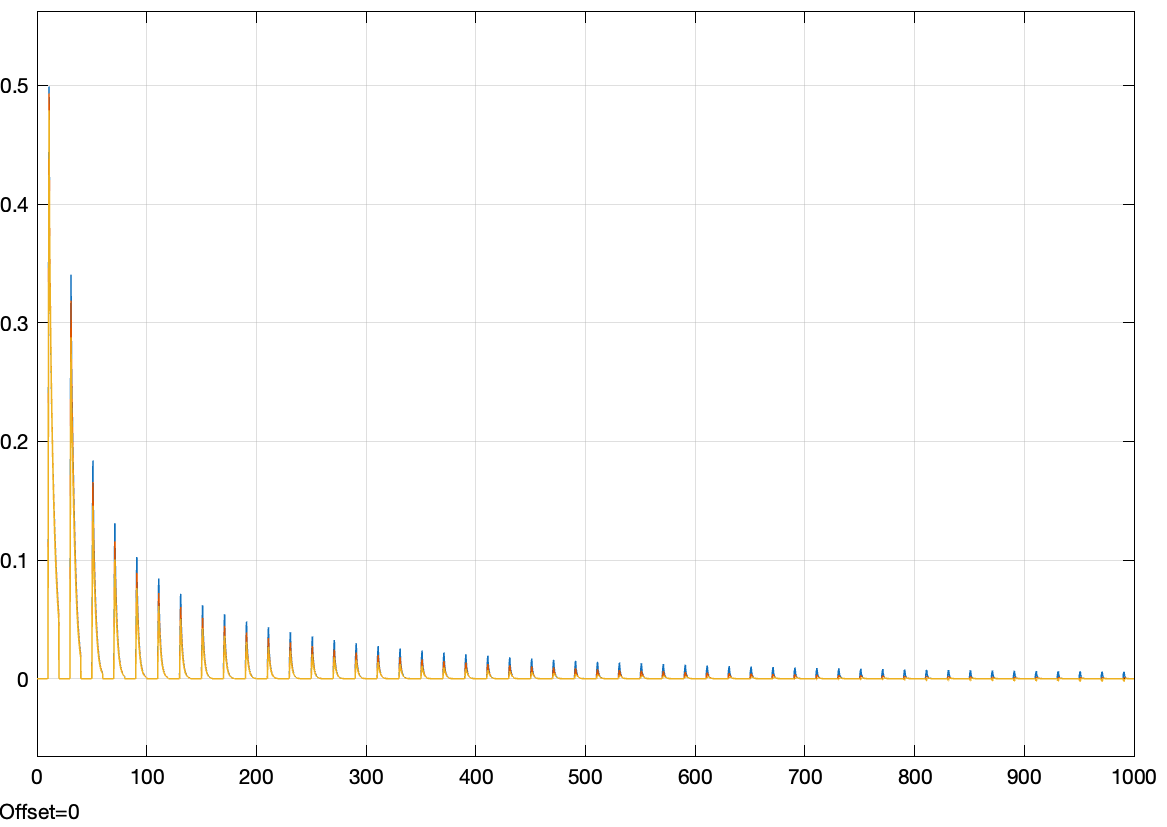
\includegraphics[width=\textwidth]{abbildungen/c_ep_approx_convergence_weight_update.png}
    \caption{Änderungsrate der Gewichte}
  \end{subfigure}%
  \hfill
  \begin{subfigure}[b]{0.3\textwidth}
    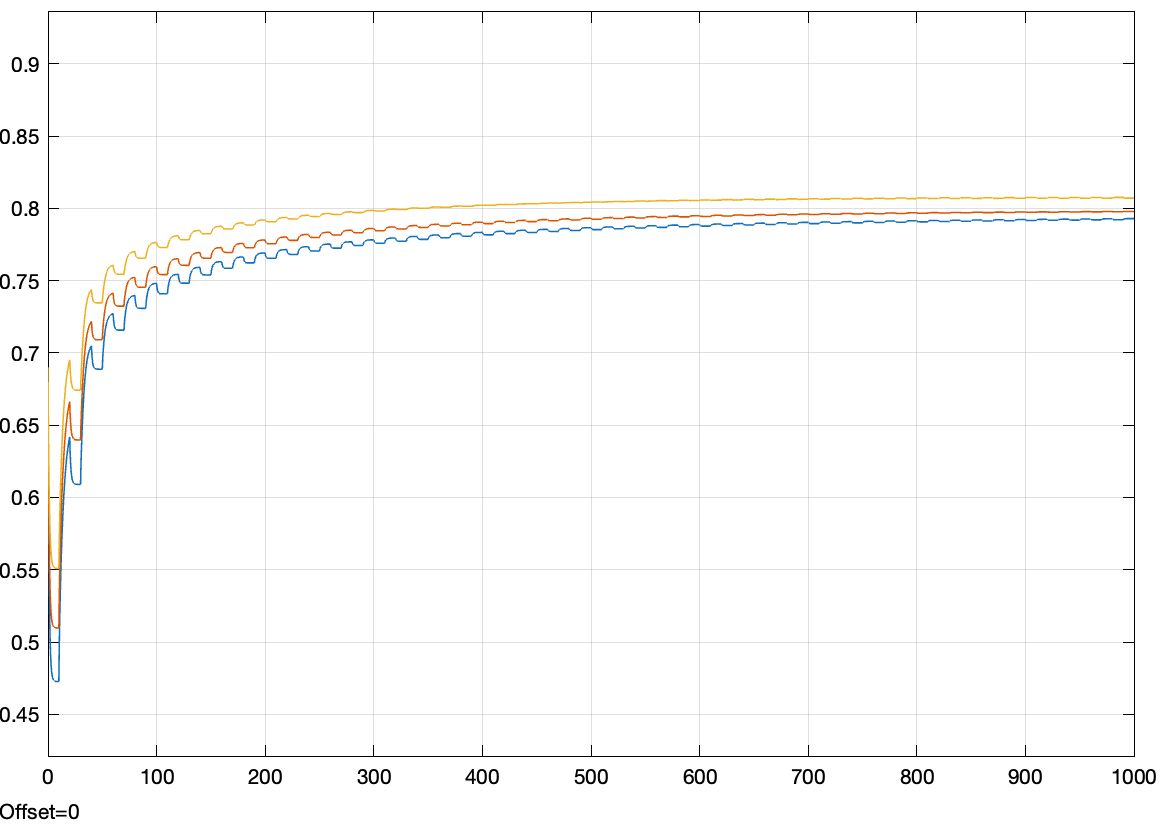
\includegraphics[width=\textwidth]{abbildungen/c_ep_approx_convergence_ausgabe.png}
    \caption{Ausgabe des Modells}
  \end{subfigure}%
  \hfill
  \begin{subfigure}[b]{0.3\textwidth}
    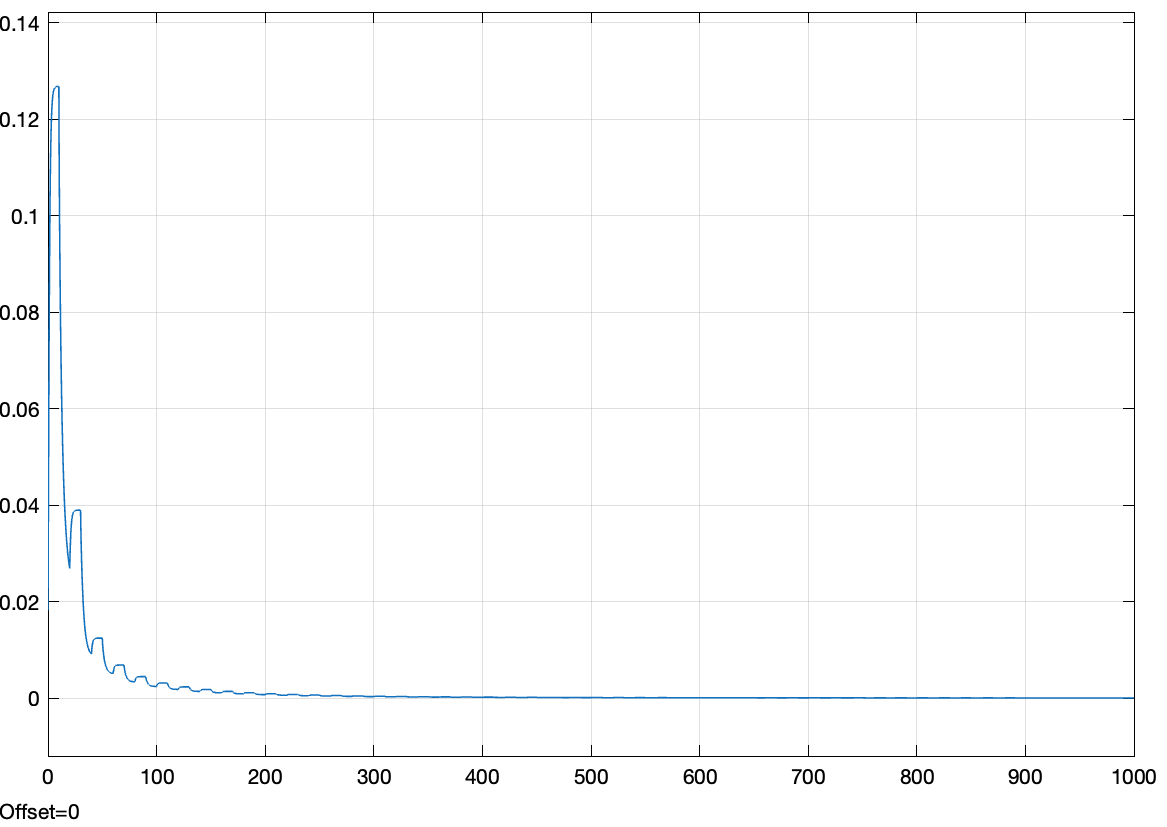
\includegraphics[width=\textwidth]{abbildungen/c_ep_approx_convergence_kosten.png}
    \caption{Kosten des Modells}
  \end{subfigure}
  \\
  Quelle: Eigene Darstellung
\end{figure}
